\documentclass[notes,10pt, aspectratio=169]{beamer}

\usepackage{pgfpages}
% These slides also contain speaker notes. You can print just the slides,
% just the notes, or both, depending on the setting below. Comment out the want
% you want.
\setbeameroption{hide notes} % Only slide
%\setbeameroption{show only notes} % Only notes
%\setbeameroption{show notes on second screen=right} % Both
\usepackage{colortbl}
\usepackage{helvet}
\usepackage[default]{lato}
\usepackage{array}
\usepackage{eurosym}
\usepackage{setspace}
\usepackage{animate}
\usepackage{multicol}
\usepackage{breqn}
\usepackage{subcaption}
\usepackage{caption}
\captionsetup{font=scriptsize, justification=raggedright,singlelinecheck=false}
\usepackage[export]{adjustbox}
\usepackage[scale=2]{ccicons}
\usepackage{tikz}
\newenvironment{wideitemize}{\itemize\addtolength{\itemsep}{10pt}}{\enditemize}
\usepackage{natbib}

\usepackage{tikz}
\usepackage{verbatim}
\setbeamertemplate{note page}{\pagecolor{yellow!5}\insertnote}
\usepackage{amsmath}
%\usepackage{mathpazo}
\usepackage{hyperref}
\usepackage{lipsum}
\usepackage{multimedia}
\usepackage{multirow}
\usepackage{graphicx}
\usepackage{dcolumn}
\usepackage{bbm}
\newcolumntype{d}[0]{D{.}{.}{5}}

\usepackage{changepage}
\usepackage{appendixnumberbeamer}
% \newcommand{\beginbackup}{
%   \newcounter{framenumbervorappendix}
%   \setcounter{framenumbervorappendix}{\value{framenumber}}
%   \setbeamertemplate{footline}
%   {
%      \leavevmode%
%      \hline
%      box{%
%       \begin{beamercolorbox}[wd=\paperwidth,ht=2.25ex,dp=1ex,right]{footlinecolor}%
% %         \insertframenumber  \hspace*{2ex} 
%       \end{beamercolorbox}}%
%      \vskip0pt%
%   }
%  }

 \setbeamertemplate{footline}{
    \hbox{%
    \begin{beamercolorbox}[wd=\paperwidth,ht=3ex,dp=1.5ex,leftskip=2ex,rightskip=2ex]{page footer}%
        %\usebeamerfont{title in head/foot}%
        %\insertshorttitle \hfill
        %\insertsection \hfill
        %\tableofcontents[currentsection] \hfill
        \insertsectionnavigationhorizontal{0.7\paperwidth}{}{} \hfill 
        \insertframenumber{} / \inserttotalframenumber
    \end{beamercolorbox}}%
}
\newcommand{\backupend}{
   \addtocounter{framenumbervorappendix}{-\value{framenumber}}
   \addtocounter{framenumber}{\value{framenumbervorappendix}} 
}

\useinnertheme[shadow]{rounded}
\setbeamercolor{block title example}{fg=black,bg=orange!50!white}
\setbeamercolor{block body example}{fg=black, bg=orange!30!white}
\setbeamercolor{block title alert}{fg=black,bg=green!50!white}
\setbeamercolor{block body alert}{fg=black, bg=green!30!white}
\setbeamercolor{block title}{use=structure,fg=structure.fg,bg=structure.fg!20!bg}
\setbeamercolor{block body}{parent=normal text,use=block title,bg=block title.bg!50!bg}

\newcommand\independent{\protect\mathpalette{\protect\independenT}{\perp}}
\def\independenT#1#2{\mathrel{\rlap{$#1#2$}\mkern2mu{#1#2}}}

\usepackage{graphicx}
\usepackage[space]{grffile}
\usepackage{booktabs}

% These are my colors -- there are many like them, but these ones are mine.
\definecolor{blue}{RGB}{0,114,178}
\definecolor{red}{RGB}{213,94,0}
\definecolor{yellow}{RGB}{240,228,66}
\definecolor{green}{RGB}{0,158,115}

\setbeamercolor{section in head/foot}{fg=blue}


\hypersetup{
  colorlinks=false,
  linkbordercolor = {white},
  linkcolor = {blue}
}


%% I use a beige off white for my background
\definecolor{MyBackground}{RGB}{255,253,218}

%% Uncomment this if you want to change the background color to something else
%\setbeamercolor{background canvas}{bg=MyBackground}

%% Change the bg color to adjust your transition slide background color!
\newenvironment{transitionframe}{
  \setbeamercolor{background canvas}{bg=yellow}
  \begin{frame}}{
    \end{frame}
}

\setbeamercolor{frametitle}{fg=blue}
\setbeamercolor{title}{fg=black}
%\setbeamertemplate{footline}[frame number]
\setbeamertemplate{navigation symbols}{} 
\setbeamertemplate{itemize items}{-}
\setbeamercolor{itemize item}{fg=blue}
\setbeamercolor{itemize subitem}{fg=blue}
\setbeamercolor{enumerate item}{fg=blue}
\setbeamercolor{enumerate subitem}{fg=blue}
\setbeamercolor{button}{bg=white,fg=blue,}



% If you like road maps, rather than having clutter at the top, have a roadmap show up at the end of each section 
% (and after your introduction)
% Uncomment this is if you want the roadmap!
% \AtBeginSection[]
% {
%    \begin{frame}
%        \frametitle{Roadmap of Talk}
%        \tableofcontents[currentsection]
%    \end{frame}
% }
\setbeamercolor{section in toc}{fg=blue}
\setbeamercolor{subsection in toc}{fg=red}
%\setbeamersize{text margin left=1em,text margin right=1em} 
\setbeamersize{text margin left=0.7cm,text margin right=0.7cm} 


\title[]{\textcolor{blue}{Lecture 8:\\Threats to Identification}}
\author{25117 - Econometrics}
\institute[shortinst]{Universitat Pompeu Fabra}

\date{November 13th, 2024}

\begin{document}

\begin{frame}[plain]
\maketitle
\end{frame}



\begin{frame}{What we learned in the last lesson}
\begin{itemize}
    \item What if the marginal effect of $X$ on $Y$ is not constant? A linear regression is misspecified: the functional form is wrong.\\
    \item We can extend the multiple OLS framework to introduce non-linearities. The effect on $Y$ of a change in the independent variable(s) can be computed by evaluating the regression function at two values of the independent variable(s).\\
    \item A polynomial regression includes powers of $X$ as regressors. A quadratic regression includes $X$ and $X^2$, and a cubic regression includes $X$, $X^2$, and $X^3$.
    \item Small changes in logarithms can be interpreted as proportional or percentage changes in a variable. Regressions involving logarithms are used to estimate proportional changes and elasticities.
    \item The product of two variables is called an interaction term. When interaction terms are included as regressors, they allow the regression slope and/or intercept of one variable to depend on the value of another variable.
\end{itemize}
\end{frame}

\begin{frame}{Classic Pitfalls to Regression Analysis}
\begin{itemize}
    \item Let’s step back and take a broader look at regression. Is there a systematic way to assess (critique) regression studies? We know the strengths of multiple regression – but what are the pitfalls?\\[1em]
    \item We will list the most common reasons that multiple regression estimates, based on observational data, can result in biased estimates of the causal effect of interest.
\end{itemize}
\begin{exampleblock}{Internal validity}
The statistical inferences about causal effects are valid for the population being studied.
\end{exampleblock}
\begin{exampleblock}{External validity}
The statistical inferences can be generalized from the population and setting studied to other populations and settings, where the ``setting'' refers to the legal, policy, and physical environment and related salient features.
\end{exampleblock}

\end{frame}

\begin{frame}{External Validity}
Assessing threats to external validity requires detailed substantive knowledge and judgment on a case-by-case basis... How far can we generalize class size results from California?\\[1em]
\begin{itemize}
    \item[$\longrightarrow$] Differences in time (California in 1999 vs California in 2023? )\\[1em]
    \item[$\longrightarrow$] Differences in space (California in 1999 vs Catalonia in 1999?)\\[1em]
    \item[$\longrightarrow$] Differences in settings (Robust across different legal and institutional requirements/frameworks?)\\[1em]
\end{itemize}
Would you expect the magnitude and direction of the effects in the 1999 California schools sample to be the same for Catalonia in 2023?\\[1em]

A comparison of many related studies on the same topic is called a meta-analysis.
\end{frame}


\begin{frame}{A Meta-Analysis -- Lane (2016)}
\begin{figure}
  \centering
         \vspace{-1mm}
         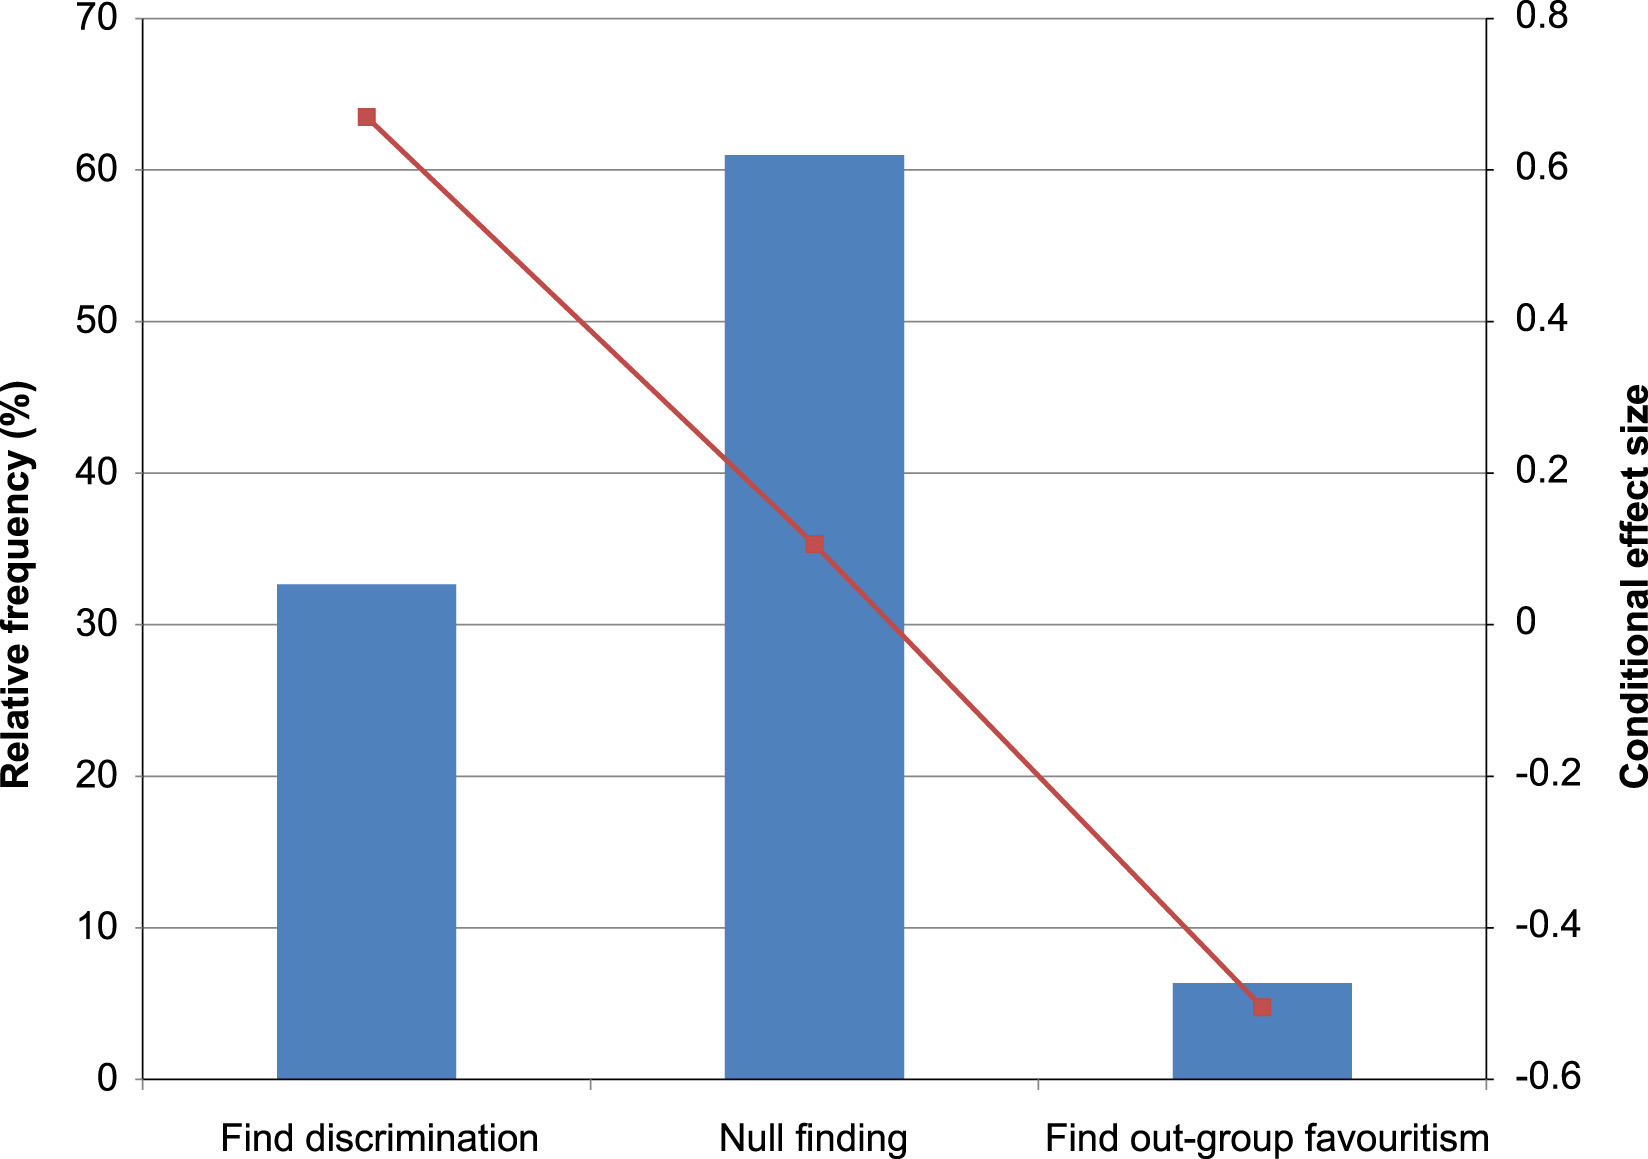
\includegraphics[scale=1.2]{images/extvalidity.jpg}
\end{figure}
\end{frame}

\begin{frame}{A Meta-Analysis -- Hahn-Holbrook et al. (2018)}
\begin{figure}
  \centering
         \vspace{-1mm}
         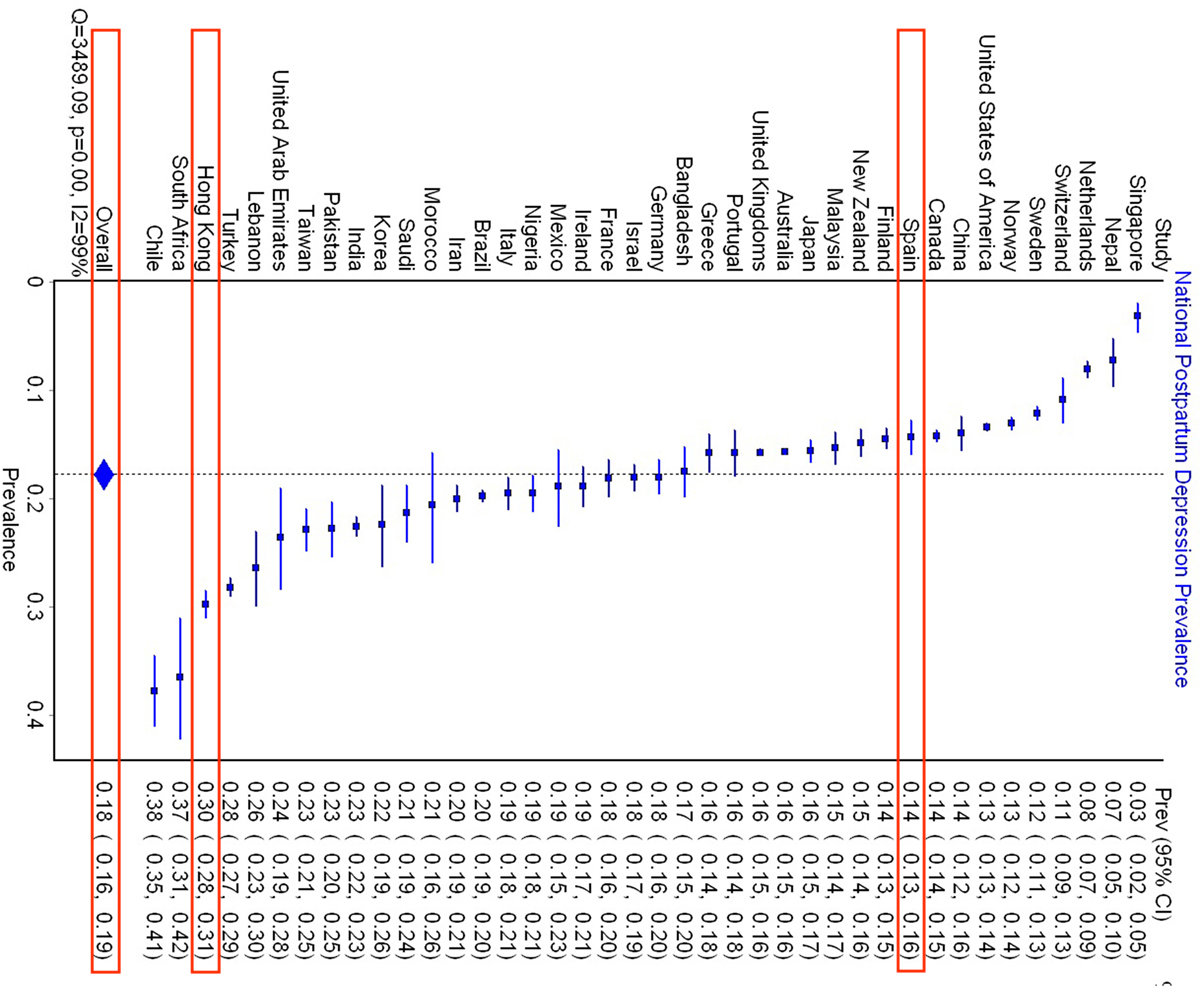
\includegraphics[width=.65\linewidth]{images/extvalidity2.jpg}
\end{figure}
\end{frame}

\begin{frame}{Internal Validity}
Are the statistical inferences about causal effects valid for the population being studied?\\[1em]
Five threats to the internal validity of regression studies:
\begin{itemize}
    \item Omitted variable bias
    \item Wrong functional form
    \item Errors-in-variables bias
    \item Sample selection bias
    \item Simultaneous causality bias
\end{itemize}
\vspace{1em}
All of these imply that $\mathbb{E}(u_i\mid X_1, X_2, \dots, X_k)\neq 0$ (or that the conditional mean independence fails) – in which case O L S is biased and inconsistent!
\end{frame}

\begin{frame}{Omitted Variable Bias (revision)}
The bias in the OLS estimator that occurs as a result of an omitted factor, or variable, is called omitted variable bias. For omitted variable bias to occur, the omitted variable $Z$ must satisfy two conditions:
\begin{enumerate}
    \item $Z$ is a determinant of $Y$ (i.e. $Z$ is part of $u$); and
    \item $Z$ is correlated with the regressor $X$ (i.e., $corr(Z,X)\neq 0)$
\end{enumerate}

\begin{center}
\begin{figure}
    \resizebox{.6\linewidth}{!}{%



\tikzset{every picture/.style={line width=0.75pt}} %set default line width to 0.75pt        

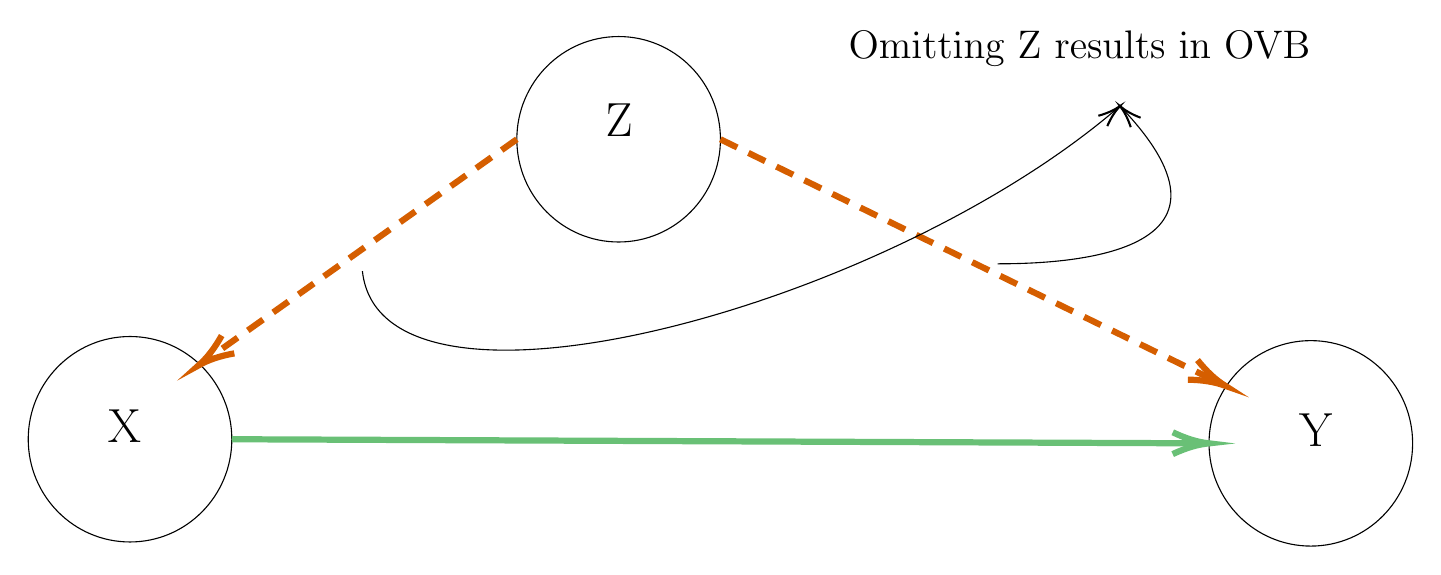
\begin{tikzpicture}[x=0.75pt,y=0.75pt,yscale=-1,xscale=1]
%uncomment if require: \path (0,285); %set diagram left start at 0, and has height of 285

%Shape: Ellipse [id:dp36615011120920427] 
\draw   (254.41,66.5) .. controls (254.41,39.16) and (276.37,17) .. (303.46,17) .. controls (330.54,17) and (352.5,39.16) .. (352.5,66.5) .. controls (352.5,93.83) and (330.54,115.99) .. (303.46,115.99) .. controls (276.37,115.99) and (254.41,93.83) .. (254.41,66.5) -- cycle ;
%Shape: Ellipse [id:dp34906029723118115] 
\draw   (19,211.02) .. controls (19,183.69) and (40.96,161.53) .. (68.04,161.53) .. controls (95.13,161.53) and (117.09,183.69) .. (117.09,211.02) .. controls (117.09,238.36) and (95.13,260.52) .. (68.04,260.52) .. controls (40.96,260.52) and (19,238.36) .. (19,211.02) -- cycle ;
%Shape: Ellipse [id:dp6974919182309072] 
\draw   (587.91,213) .. controls (587.91,185.67) and (609.87,163.51) .. (636.96,163.51) .. controls (664.04,163.51) and (686,185.67) .. (686,213) .. controls (686,240.34) and (664.04,262.5) .. (636.96,262.5) .. controls (609.87,262.5) and (587.91,240.34) .. (587.91,213) -- cycle ;
%Straight Lines [id:da04124970397057681] 
\draw [color={rgb, 255:red, 126; green, 211; blue, 33 }  ,draw opacity=1 ][line width=2.25]    (117.09,211.02) -- (583.91,212.99) ;
\draw [shift={(587.91,213)}, rotate = 180.24] [color={rgb, 255:red, 126; green, 211; blue, 33 }  ,draw opacity=1 ][line width=2.25]    (17.49,-5.26) .. controls (11.12,-2.23) and (5.29,-0.48) .. (0,0) .. controls (5.29,0.48) and (11.12,2.23) .. (17.49,5.26)   ;
%Straight Lines [id:da035209354566531736] 
\draw [color={rgb, 255:red, 255; green, 0; blue, 0 }  ,draw opacity=1 ][line width=2.25]  [dash pattern={on 6.75pt off 4.5pt}]  (254.41,66.5) -- (104.26,173.18) ;
\draw [shift={(101,175.5)}, rotate = 324.6] [color={rgb, 255:red, 255; green, 0; blue, 0 }  ,draw opacity=1 ][line width=2.25]    (17.49,-5.26) .. controls (11.12,-2.23) and (5.29,-0.48) .. (0,0) .. controls (5.29,0.48) and (11.12,2.23) .. (17.49,5.26)   ;
%Straight Lines [id:da19389419961485554] 
\draw [color={rgb, 255:red, 255; green, 0; blue, 0 }  ,draw opacity=1 ][line width=2.25]  [dash pattern={on 6.75pt off 4.5pt}]  (352.5,66.5) -- (592.16,183.53) ;
\draw [shift={(595.76,185.29)}, rotate = 206.03] [color={rgb, 255:red, 255; green, 0; blue, 0 }  ,draw opacity=1 ][line width=2.25]    (17.49,-5.26) .. controls (11.12,-2.23) and (5.29,-0.48) .. (0,0) .. controls (5.29,0.48) and (11.12,2.23) .. (17.49,5.26)   ;
%Curve Lines [id:da92152652585756] 
\draw    (486,126.5) .. controls (518.84,126.5) and (613.05,122.54) .. (546.02,51.57) ;
\draw [shift={(545,50.5)}, rotate = 46.22] [color={rgb, 255:red, 0; green, 0; blue, 0 }  ][line width=0.75]    (10.93,-3.29) .. controls (6.95,-1.4) and (3.31,-0.3) .. (0,0) .. controls (3.31,0.3) and (6.95,1.4) .. (10.93,3.29)   ;
%Curve Lines [id:da6333756929191379] 
\draw    (180,130) .. controls (189,213) and (432,148.5) .. (545,50.5) ;
\draw [shift={(545,50.5)}, rotate = 139.07] [color={rgb, 255:red, 0; green, 0; blue, 0 }  ][line width=0.75]    (10.93,-3.29) .. controls (6.95,-1.4) and (3.31,-0.3) .. (0,0) .. controls (3.31,0.3) and (6.95,1.4) .. (10.93,3.29)   ;

% Text Node
\draw (56.08,195.51) node [anchor=north west][inner sep=0.75pt]   [align=left] {{\LARGE X}};
% Text Node
\draw (295.97,47.97) node [anchor=north west][inner sep=0.75pt]   [align=left] {{\LARGE Z}};
% Text Node
\draw (630.08,197.51) node [anchor=north west][inner sep=0.75pt]   [align=left] {{\LARGE Y}};
% Text Node
\draw (413,13) node [anchor=north west][inner sep=0.75pt]  [font=\Large] [align=left] {Omitting Z results in OVB};


\end{tikzpicture}

}
\end{figure}
\end{center}

If the multiple regression includes control variables, then we need to ask whether there are omitted factors that are not adequately controlled for, that is, whether the error term is correlated with the variable of interest even after we have included the control variables.
\end{frame}

\begin{frame}{Solutions to OVB}

\begin{itemize}
    \item If the omitted causal variable can be measured, include it as an additional regressor in multiple regression;\\[1em]
    \item If you have data on one or more controls and they are adequate (that is, if conditional mean independence plausibly holds), then include the control variables;\\[1em]
    \item If the omitted variable(s) cannot be measured or adequately controlled for, use instrumental variables regression ($Lecture~9$);\\[1em]
    \item Possibly, use panel data in which each entity (individual) is observed more than once ($Lecture~10$);\\[1em]
    \item Run a randomized controlled experiment if you can (again, randomization of treatment $X$ ensures that $X$ necessarily will be distributed independently of $u$.)
\end{itemize}
\end{frame}




\begin{frame}{Wrong Functional Form (revision)}
 \begin{columns}
\begin{column}{0.45\textwidth}
Arises if the functional form is incorrect -- e.g., an interaction term is incorrectly omitted; then inferences on causal effects will be biased.\\[1em]

\textbf{Solutions to functional form mispecification:}
\begin{itemize}
    \item Continuous dependent variable: use the “appropriate” nonlinear specifications in $X$ (logarithms, interactions, etc.) ($last~lecture$)
    \item Discrete (example: binary) dependent variable: need an extension of multiple regression methods (``probit'' or ``logit'' analysis for binary dependent variables). ($Lecture~11$)
\end{itemize}

\end{column}
\begin{column}{0.6\textwidth}
\begin{figure}
  \centering
         \vspace{-2mm}
        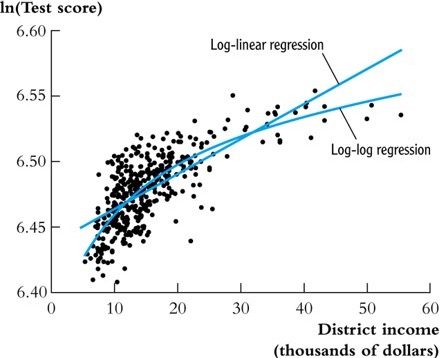
\includegraphics[scale=.5]{images/loglog.jpg}
\end{figure}
\end{column}
\end{columns}
\end{frame}



\begin{frame}{Errors-in-variables}
So far we have assumed that $X$ is measured without error.\\[1em]

In reality, economic data often have measurement error
\begin{itemize}
    \item Data entry errors in administrative data
    \item Recollection errors in surveys (when did you start your current job?)
    \item Ambiguous questions (what was your income last year?)
    \item Intentionally false response problems with surveys (What is the current value of your financial assets? How often do you drink and drive?)
\end{itemize}
\vspace{1em}
Now consider $\tilde{X}$, the mis-measured version of X (which is the actually observed data) vs $X$, the true, unobserved value of your treatment...
\end{frame}

\begin{frame}{Errors-in-variables}
You think you are running
\begin{equation*}
    Y_i = \beta_0 + \beta_1 X_i + u_i
\end{equation*}
But because $X$ is mis-measured, you are actually running
\begin{equation*}
    Y_i = \beta_0 + \beta_1 \tilde{X}_i + [\beta_1 (X-\tilde{X}) + u_i]
\end{equation*}
i.e., since $X-\tilde{X}$ is unobserved,
\begin{equation*}
    Y_i = \beta_0 + \beta_1 \tilde{X}_i + \tilde{u}_i
\end{equation*}
where $\tilde{u}_i=\beta_1 (X-\tilde{X}) + u_i$..\\[1em]

Therefore,
\begin{equation*}
    cov(\tilde{X}_i, \tilde{u}_i) = \beta_1 cov(\tilde{X}_i, X_i-\tilde{X}_i) + cov(\tilde{X}_i, u_i)
\end{equation*}
It is often plausible that $cov(\tilde{X}_i, u_i)=0$, but typically $cov(\tilde{X}_i, X-\tilde{X})\neq 0$, and therefore, $cov(\tilde{X}_i, \tilde{u}_i) \neq 0$... yielding a biased $\hat{\beta_1}$.


\end{frame}

\begin{frame}{Classical Measurement Error}
The classical measurement error model assumes that $\tilde{X}_i=X_i+v_i$ where $v_i$ is is mean-zero random noise (e.g., white noise) with $\rho_{X_i, v_i}=0$ and $\rho_{u_i, v_i}=0$.\\[1em]

Under the classic measurement error model, $\hat{\beta}_1$ will be biased towards zero...\\[1em]

Intuitively: Take the true variable and add a very large amount of random noise. In the limit, $\tilde{X}_i$ will be completely unrelated to $Y_i$ so $\mathbb{E}(\hat{\beta}_1)$ is zero...\\[1em]

Before reaching this limit, the relationship between  $\tilde{X}_i$ and $Y_i$ will be toned down, biasing $\hat{\beta}_1$ towards zero.\\[1em]

\end{frame}

\begin{frame}{Classical Measurement Error}
Starting from,
\begin{eqnarray*}
    cov(\tilde{X}_i, \tilde{u}_i) = \beta_1 cov(\tilde{X}_i, X_i-\tilde{X}_i) + cov(\tilde{X}_i, u_i)
\end{eqnarray*}
Then, for $\tilde{X}_i=X_i+v_i$,  with $\rho_{X_i, v_i}=0$ and $\rho_{u_i, v_i}=0$,
\begin{eqnarray*}
        &cov(\tilde{X}_i, \tilde{u}_i) &= \beta_1 cov(X_i+v_i, -v_i)=-\beta_1\sigma_v^2\\
        &var(\tilde{X}_i)&=\sigma_X^2 + \sigma_v^2
\end{eqnarray*}
And back to basics:
\begin{eqnarray*}
        &\hat{\beta}_1 \overset{p}{\to} & \beta_1 + \frac{cov(\tilde{X}_i, \tilde{u}_i)}{var(\tilde{X}_i)}\\
        & {} &= \beta_1 -\beta_1\frac{\sigma_v^2}{\sigma_X^2 + \sigma_v^2} = \beta_1  \frac{\sigma_X^2}{\sigma_X^2 + \sigma_v^2}
\end{eqnarray*}
so $\hat{\beta}_1$ will be biased towards 0, even in large samples, and even approximate zero if the noise's variance is large enough.
\end{frame}

\begin{frame}{Missing Data}
Data are often missing. Sometimes missing data introduces bias, sometimes it doesn’t. It is useful to consider three cases:
\begin{enumerate}
    \item Data are missing at random.
    \item Data are missing based on the value of one or more $X$’s
    \item Data are missing based in part on the value of Y or u
\end{enumerate}
\vspace{1em}
Cases 1 and 2 don’t introduce bias: the standard errors are larger than they would be if the data weren’t missing, but $\hat{\beta}_k$ is unbiased.

\textbf{\textit{Case 1:}} Suppose you took a random sample of 100 workers and recorded their answers, but your dog randomly ate 20 of the response sheets. This is equivalent to having taken a simple random sample of 80 workers, so no bias is introduced.

\vspace{0.5em}
\textbf{\textit{Case 2:}} In the test scores exercise, suppose you do not observe schools with a share of subsidized meals below $40\%$. You cannot draw conclusions for those schools, but you can still draw conclusions about the subset with a share of subsidized meals at least $40\%$.

\vspace{0.5em}
\textbf{\textit{Case 3}} introduces sample selection bias.

\end{frame}

\begin{frame}{Sample Selection Bias}

\begin{block}{Sample selection bias}
Bias that arises when a selection process \textbf{a)} influences the availability of data, and  \textbf{b)} is related to the dependent variable beyond depending on the regressors.
\end{block}
\vspace{1em}
\textbf{Fictuous Simple Example:} you want to estimate the average males' height in Barcelona. To collect your data, you go to the Palau Blaugrana and record the heights of the basketball team. Formally, you have sampled individuals in a way that is related to the outcome $Y$ (height), which results in bias.

\vspace{1em}

\textbf{Real Example:} In 1936, the Literary Gazette published a poll predicting that presidential candidate Landon would win by a landslide against Roosevelt. The opposite happened: Roosevelt won with 60.8\% of the votes. It turned out that the Literary Gazette had sampled phone records from automobile registration files. In 1936, people owning a car and a telephone were richer, and more likely Republicans... supporting Landon.

\vspace{1em}

\textbf{Solution:} Avoid it in the first place. If you cannot, some methods for estimating models with sample selection exist (not now,  a bit discussed in $Lecture~11$).
\end{frame}

\begin{frame}{Simultaneity Bias}
\begin{block}{Simultaneity Bias}
Also called simultaneous equations bias. It arises in a regression of $Y$ on $X$ when, in addition to the causal link of interest from $X$ to $Y$, there is a causal link from $Y$ to $X$. This reverse causality makes $X$ correlated with the error term in the population regression of interest.
\end{block}
\vspace{1em}
\textbf{California Example:} The share of subsidised meals affects schools test scores. But schools with higher test scores might be allocated more resources, allowing them to subsidise more meals.

\vspace{1em}

Consider the following system of simultaneous equations:
\begin{eqnarray*}
    &Y_i &= \beta_0 + \beta_1 X_i + u_i\\
    &X_i &= \gamma_0 + \gamma_1 Y_i + v_i
\end{eqnarray*}
$X_i$ is a function of $u_i$, the unexplained variation of $Y_i$.

\vspace{1em}

\textbf{Solution:} Mostly RCT or IV methods ($Lecture~9$).
\end{frame}


\begin{frame}
\frametitle{Inconsistent Standard Errors}

\begin{itemize}
  \item Inconsistent standard errors can impact the internal validity of a multiple regression study.\\[1em]
  \item Even with consistent OLS estimators and large samples, inconsistent standard errors lead to hypothesis tests with incorrect significance levels and unreliable 95\% confidence intervals.\\[1em]
  \item Main reasons for inconsistent standard errors:
    \begin{itemize}
      \item \textbf{Heteroskedasticity:} For historical reasons, most regression software report by defaulkt homoskedastic-only standard errors. Use heteroskedasticity-robust standard errors and F-statistics with a heteroskedasticity-robust variance estimator.\\[.5em]
      \item \textbf{Correlation of the Error Term Across Observations:} E.g., if the omitted variables that constitute the regression error are persistent (like district demographics or geographies), these omitted variables could result in serial and/or spatial correlation of the regression errors for adjacent observations. Common in panel data or time series data, requires alternative formulas for standard errors. (more in $Lecture~10$)
    \end{itemize}
    \vspace{1em}
  \item Addressing these issues is crucial for maintaining internal validity.

\end{itemize}
\end{frame}

\begin{frame}{Internal Validity Checklist for Multiple Variables Regressions}
Applying this list of threats to a multiple regression study provides a systematic way to assess the internal validity of that study.\\[1em]
\begin{columns}
\begin{column}{0.45\textwidth}
\textbf{$\mathbb{E}(u\mid X)\neq 0$ :}
\begin{enumerate}
    \item Omitted variables
    \item Functional form misspecification
    \item Errors in variables (measurement error in the regressors)
    \item Sample selection
    \item Simultaneous causality
\end{enumerate}
\end{column}
\begin{column}{0.45\textwidth}
\textbf{Inconsistent SE :}
\begin{enumerate}
    \item Heteroskedasticity
    \item Serial and Spatial Correlation
    \item[]
    \item[]
    \item[]
\end{enumerate}
\end{column}
\end{columns}
\end{frame}

\begin{frame}{What about prediction?}
Prediction and estimation of causal effects are quite different objectives.\\[1em]
For prediction:
\begin{enumerate}
    \item The data used to estimate the prediction model must be \textit{from the same distribution} as the out-of-sample observation for which the prediction is made. This is an external validity requirement for a prediction model.
    \item The predictors should be ones \textit{that substantially contribute to explaining the variation in $Y$}. They do not need to have direct causal interpretations, and the regression coefficients in general need not estimate causal effects.
    \item The estimator must be one that produces \textit{reliable out-of-sample predictions}. When the number of regressors (predictors) is small relative to the number of observations, OLS can be used. But when the number of predictors is large, there are better estimators than OLS -- ones developed specially for the prediction problem (Big Data techniques, beyond the scope of this course).
\end{enumerate}
\end{frame}


\begin{frame}[allowframebreaks]{Material}
\begin{itemize}
    \item[--] \textbf{Textbooks:}
    \begin{itemize}
        \item Introduction to Econometrics, 4th Edition, Global Edition, by Stock and Watson -- Chapter 9
    \end{itemize}
\end{itemize}
\end{frame}


\end{document}
